\section{Results}
\label{sec:results}
We report results for models using different retrieval mechanisms and prompting styles, then provide some analysis and insight into model performance and difficulty.
We summarize models' performance using BM25 retrieval in Table~\ref{table:main-results}. 
Across the board, models struggle significantly to resolve issues.
The best performing model, Claude 2, is only able to resolve $1.96\%$ of the issues.

To analyze the importance of the retriever to the overall system results, we present the ``oracle'' retrieval results in Appendix Table~\ref{table:main-results-oracle}. There, Claude 2 is able to resolve $4.8\%$ of issues using the ``oracle'' retriever. We further analyze the importance of context in the discussion below. 

\begin{table}
\centering
\caption{
We compare models against each other using the BM25 retriever as described in Section~\ref{sec:experimental-setup}.
}
\begin{tabular}{lcccc}
\toprule
& \multicolumn{2}{c}{SWE-bench} & \multicolumn{2}{c}{SWE-bench Lite} \\
\cmidrule(lr){2-3} \cmidrule(lr){4-5}  % Add rules under the multi-columns for clarity
Model & \% Resolved & \% Apply & \% Resolved & \% Apply \\
\midrule
Claude 3 Opus   & {\bf 3.79} & 46.56        & {\bf 4.33} & {\bf 51.67} \\
Claude 2        & 1.97       & 43.07        & 3.00       & 33.00       \\
ChatGPT-3.5     & 0.17       & 26.33        & 0.33       & 10.00       \\ 
GPT-4-turbo     & 1.31       & 26.90        & 2.67       & 29.67       \\
SWE-Llama 7b    & 0.70       & 51.74        & 1.33       & 38.00       \\
SWE-Llama 13b   & 0.70       & {\bf 53.62}  & 1.00       & 38.00       \\
\bottomrule
\end{tabular}
\label{table:main-results}
\end{table}


\begin{figure}[t]
    \centering
    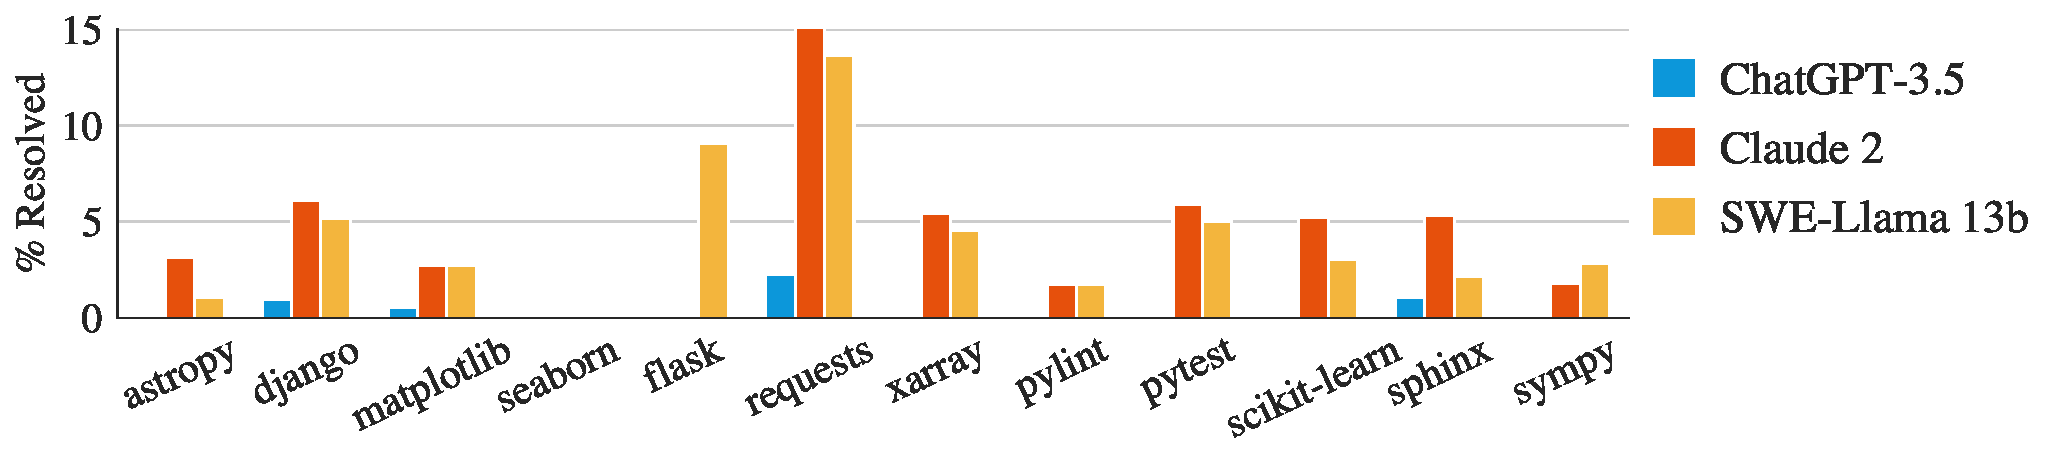
\includegraphics[width=\textwidth]{figures/assets/per_repo_oracle_fig.pdf}
    \caption{
    Resolution rate for three models across the 12 repositories represented in \benchmark{} in the ``Oracle" retrieval setting.
    }
    \label{fig:per-repo-oracle-fig}
\end{figure}

\textbf{Difficulty differs across repositories.}
When breaking performance down by repository, all models trend similarly across different repositories as show in Figure~\ref{fig:per-repo-oracle-fig}.
Despite this, the issues resolved by each model do not necessarily overlap extensively.
For example, in the ``oracle" setting Claude 2 and \swellama{} 13b perform comparably, with each model resolving $110$ and $91$ instances respectively. Yet of these instances, Claude 2 only solves $42\%$ of the instances solved by \swellama{}.

This may also be related to the presence of images in issues, which can be encoded into the issue markdown with embedded image links (i.e. \lstinline{![image][https://...]}). Some repositories naturally feature more instances with images; for example $32$\% of matplotlib and $10$\% of seaborn instances contain embedded images in their issue text compared to just $2$\% of all instances. Solving these instances may require multi-modal LMs or some kind of external tool use to process images.

\textbf{Difficulty correlates with context length.}
Chat models may be pre-trained on long sequences of code but are typically asked to generate shorter coder snippets with limited context provided to frame the question.
As shown in Figure~\ref{fig:performance-vs-context-length}, we see that as total context length increases, Claude 2's performance drops considerably; behavior that is also observed in other models.
In our evaluation settings, models see a lot of code that may not be directly related to solving the issue at hand, and they seem to frequently struggle with localizing problematic code needing to be updated.
This result corroborates other studies showing that models become distracted by additional context and may be sensitive to the relative location of target sequences~\citep{liulostinthemiddle}.
Even when increasing the maximum context size for BM25 would increase recall with respect to the oracle files, performance drops, as shown in Table~\ref{table:bm25-results}, as models are simply ineffective at localizing problematic code.

\begin{figure}[!htb]
\begin{minipage}{0.64\linewidth}
    \centering
    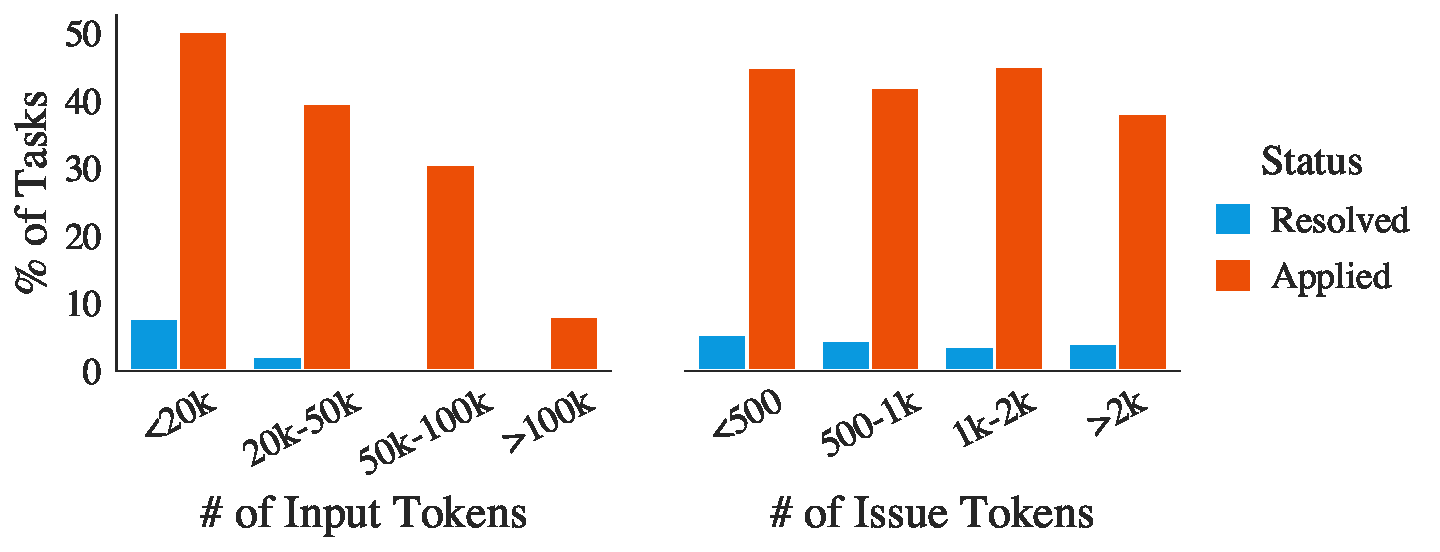
\includegraphics[width=0.98\textwidth]{figures/assets/swellama-issue-length-tokens.pdf}
    \captionof{figure}{We compare the performance of Claude 2 on tasks partitioned by total input length and by only the issue length.}
    \label{fig:performance-vs-context-length}
\end{minipage}%
\hfill
\begin{minipage}{0.34\linewidth}
\captionof{table}{We show the results for the ``Oracle"-collapsed retrieval setting, which uses oracle files but collapses code that isn't directly modified by the PR $\pm 15$  lines.}
\resizebox{\textwidth}{!}{
\begin{tabular}{lcc}
    \toprule
    \multirow{2}{*}{Model} & \multicolumn{2}{c}{``Oracle"-collapsed} \\
    \cmidrule(lr){2-3}
    & Resolved & Applied \\
    \midrule
    Claude 3 Opus & {\bf 9.39} & 48.00       \\
    Claude 2      & 5.93       & {\bf 68.18} \\
    GPT-4         & 3.40       & 48.65       \\
    ChatGPT-3.5   & 1.09       & 40.93       \\
    \bottomrule
\end{tabular}
}
\label{table:editonly-results}
\end{minipage}
\end{figure}

Further investigating this, we provide an input ablation on the ``oracle'' retrieval context, ``oracle''-collapsed, where retrieved files are collapsed entirely, except for the lines actually edited by the true pull request (with $\pm15$ lines of buffer) shown in Table~\ref{table:editonly-results}. In this setting, we see increases in performance, with GPT-4 jumping from $1.3\%$ to $3.4\%$ and Claude 2 from $4.8\%$ to $5.9\%$.

\textbf{Difficulty does not correlate with issue resolution date.}
In Table~\ref{table:temporal-results} we show model results in the ``oracle" retrieval setting, partitioned by date, for PRs created before or after 2023.
We find that for most models there's little difference in performance before or after this date, with the exception of GPT-4.
We consider this result to be largely promising as it suggests that despite models having been exposed to some version of an repository's codebase, they are unlikely to ``cheat'' to address issues simply by generating a more recent version of the repository.

\begin{table}[ht]
\centering
\caption{
We compare performance on task instances from before and after 2023 in the ``Oracle" retrieval setting.
Most models show little difference in performance. $^*$Due to budget constraints, GPT-4 is evaluated on a $25\%$ random subset of \benchmark{} tasks, which may impact performance.
}
\begin{tabular}{lccccc}
\toprule
    & Claude 2   & ChatGPT-3.5 & GPT-4$^*$  & SWE-Llama 7b & SWE-Llama 13b \\
\midrule
    Before 2023 & {\bf 4.87} & 0.49        & {\bf 1.96} & 2.95         & {\bf 3.98} \\
    After 2023   & 4.23       & {\bf 0.77}  & 0.0        & {\bf 3.46}   & {3.85} \\
\bottomrule
\end{tabular}
\label{table:temporal-results}
\end{table}

\textbf{Finetuned models are sensitive to context distribution shifts.}
The finetuned models \swellama{} 7b and 13b perform surprisingly poorly with BM25 retrieved context.
As these models were finetuned using the ``oracle" retrieval as context, we suspect this shift in context makes it difficult for the model to perform reliably.
For instance, \swellama{} was trained to edit every file included as context whereas in the BM25 setting many files provided in context are not expected to be changed.

\textbf{Generating patches is easier than generating whole files.}
Models are often trained using standard code files and likely rarely see patch files. 
We generally formulate our task to have models generate patch files as opposed to recreating the entire file with their proposed change, since patch files will usually be a much more efficient representation of a file change.
As shown in Table~\ref{table:main-results}, we observe that models still struggle with generating well-formatted patch files.
So we experiment with asking models to instead regenerate entire files with their proposed changes to resolve the issue.
In this setting, we find that models generally perform worse at this task than when generating patch files; for instance, Claude 2 scores at $2.2\%$ compared to $4.8\%$ in the main table for ``oracle" retrieval.
Even when controlling for instance length, generating on the shorter half of the task instances by input tokens yields $3.9\%$ compared to $7.8\%$ for generating patches with Claude 2.

\textbf{Language models tend to generate shorter, simpler edits.}
Model generated patch files tend to add and remove fewer lines than their respective gold patch.
As shown in Table~\ref{table:quantitative-analysis-gens}, compared to an average gold patch, model generated patch files that apply correctly are less than half the total length ($74.5$ versus $30.1$ lines) of gold edit patch files, and rarely edit more than a single file.

\begin{table}[ht]
\centering
\caption{
Average edits of model generated patches in the ``oracle'' retrieval setting across successfully applied patches.
For the task instances specific to each model, we calculate the same statistics across the gold patches.
Avg Gold shows statistics macro-averaged over each models' respective gold patches.
All Gold shows statistics for all gold patches unconditioned on model performance.
}
\resizebox{0.7\textwidth}{!}{
\begin{tabular}{lccccc}
\toprule
    Model & Total Lines & Added & Removed & Functions & Files \\ \cmidrule(lr){1-1} \cmidrule(lr){2-6}  
    Claude 2 & 19.6 & 4.2 & 1.9 & 1.1 & 1.0 \\
    \quad Gold & 44.1 & 12.0 & 5.8 & 2.1 & 1.2 \\
\midrule
    ChatGPT-3.5 & 30.1 & 3.8 & 2.7 & 1.6 & 1.0 \\
    \quad Gold & 39.6 & 9.5 & 6.1 & 1.9 & 1.2 \\
\midrule
    GPT-4 & 20.9 & 4.4 & 1.5 & 1.0 & 1.0 \\
    \quad Gold & 33.6 & 8.4 & 3.8 & 1.9 & 1.1 \\
\midrule
    SWE-Llama 13b & 17.6 & 1.6 & 1.2 & 1.2 & 1.1 \\
    \quad Gold & 37.8 & 10.0 & 4.4 & 1.9 & 1.1 \\
\midrule
    SWE-Llama 7b & 16.7 & 1.3 & 1.2 & 1.2 & 1.1 \\
    \quad Gold & 40.2 & 11.3 & 4.9 & 1.9 & 1.1 \\
\midrule
    Avg Gold & 39.1 & 10.2 &  5.0 & 1.9 & 1.1 \\
    All Gold & 74.5 & 22.3 & 10.5 & 3.0 & 1.7 \\
\bottomrule
\end{tabular}
}
\label{table:quantitative-analysis-gens}
\end{table}

\subsection{A Qualitative Analysis of \swellama{} Generations}
\label{sec:results:quality-study}
We select $11$ generations from \swellama{} and Claude 2 to better understand the quality of the task and generated patches under the ``oracle" retrieval setting.
Here we discuss an example from \swellama{} and our overall findings, with in-depth analyses for other examples shown in Appendix~\ref{appx:extra-results:quality-in-depth}.

\begin{figure}[ht]
    \centering
    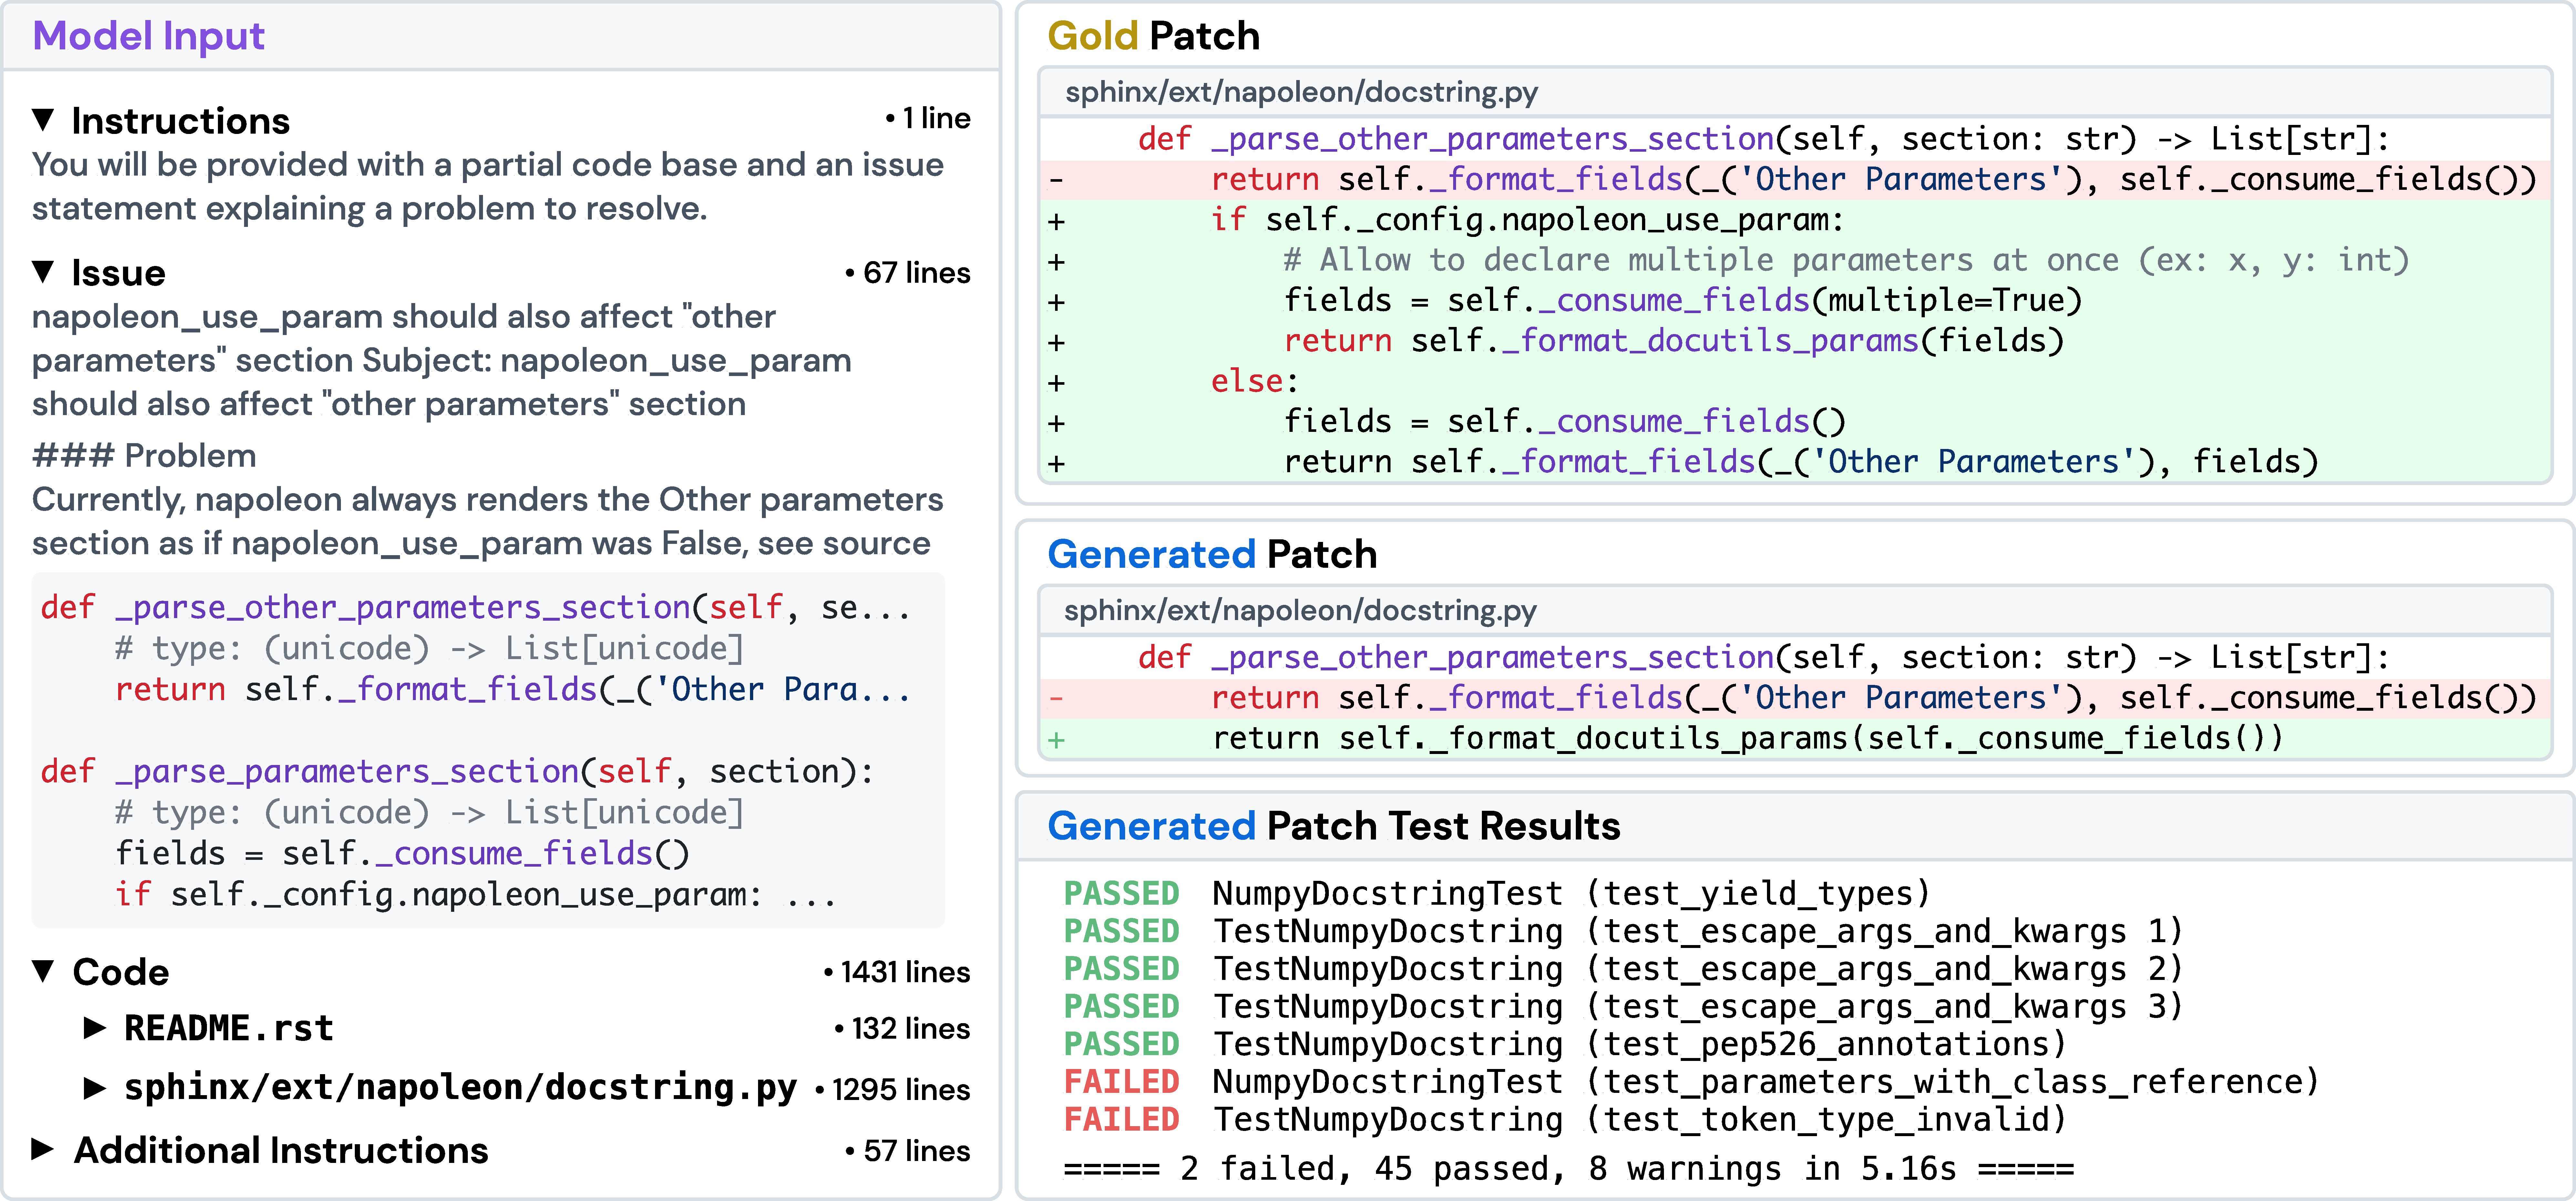
\includegraphics[width=\textwidth]{figures/assets/case-study.pdf}
    \caption{
    We show an example of an formatted task instance, a model prediction, and the testing framework logs.
    In the patches, red highlights are deletions.
    Green highlights are additions.
    }
    \label{fig:case-study}
\end{figure}

We'll consider the task instance \texttt{sphinx-doc\_\_sphinx-8713} from the Sphinx documentation generator, shown in Figure~\ref{fig:case-study}.
The issue states that the \texttt{napoleon} extension of Sphinx is not properly formatting the documentation keyword ``Other Parameters'' when the config setting \pythoninline{napoleon.use\_param} is set to \texttt{True}.
The issue text further provides a detailed code snippet of where the problematic source code is suspected to be, as well as some code examples for reproducing the error and additional information related to package versions.
For this particular instance, the model did not resolve the task, failing to pass some of the tests resolved by the gold solution.

In the ``oracle" retrieval setting, the model input provides this issue text along with some instructions, the full contents of files edited by the gold patch, and an example of the diff format we expect the answer to be in.
The total model input consists of $\num{1558}$ lines of context or $\num{20882}$ tokens. When comparing the gold patch and the model's patch, we find an obvious mistake.
While the model edits the correct function, \pythoninline{_parse_other_parameters_section} at line $684$ in \pythoninline{sphinx/ext/napoleon/docstring.py}, it changes the function to behave as if \pythoninline{napoleon.}\pythoninline{use_param} were always \texttt{True} instead of checking the config setting first and copying what the \pythoninline{_parse_parameters_section} does, like the gold patch.
In the tests, \pythoninline{test_parameters}\pythoninline{_with_class_reference} directly compares the documentation produced using a config where \pythoninline{napoleon_use_param} is set to \texttt{False}, which catches the model's error immediately.

Comparing results across all the examples we consider, we notice a few prominent trends in behavior.
Models tend to write primitive Python code and do not leverage existing third-party libraries or the rest of the codebase for their solutions.
Models' generations also reflect a ``greedy" approach of solving the problem \textit{exactly}, with little regard for code style or logical constraints that might be reflected by the codebase (i.e. using relative instead of absolute imports).
In contrast, we observe that many gold patches will make structural improvements that cover a much larger scope of the codebase; these edits not only resolve the issue, but also anticipate and solve potential future issues.
